\documentclass[conference]{IEEEtran}
\IEEEoverridecommandlockouts
% The preceding line is only needed to identify funding in the first footnote. If that is unneeded, please comment it out.
\usepackage{cite}
\usepackage{amsmath,amssymb,amsfonts}
\usepackage{algorithmic}
\usepackage{graphicx}
\usepackage{textcomp}
\usepackage{xcolor}
\def\BibTeX{{\rm B\kern-.05em{\sc i\kern-.025em b}\kern-.08em
    T\kern-.1667em\lower.7ex\hbox{E}\kern-.125emX}}
\begin{document}

\title{Metrological Characterization and Cost-Function Optimization of EMA Filters on AHT10 Environmental Transducers
}

\author{\IEEEauthorblockN{Muhammad Fauzan Faturosi}
\IEEEauthorblockA{\textit{Department of Physics} \\
\textit{Universitas Pembangunan Nasional "Veteran" Jawa Timur}\\
Surabaya, Indonesia \\
f7629118@gmail.com}
}

\maketitle

\begin{abstract}
  Accurate microclimate environmental measurements using low-cost transducers, such as the AHT10 capacitive sensor, are frequently compromised by inherent hardware noise and thermal anomalies. 
  This study investigates the metrological characterization of the measurement chain and the optimization of digital signal filtering utilizing the Exponential Moving Average (EMA) algorithm. 
  To eliminate external thermal coupling (Joule heating) and cross-interference originating from the ESP32 microcontroller's integrated radio frequency (RF) module, data acquisition was strictly executed via hardware-timer deterministic sampling at a constant interval of $\Delta t = 2.051$ seconds with all wireless protocols fully disabled.
  Steady-state characterization within an isolated chamber yielded a pure baseline noise floor with a standard deviation of $\sigma = 0.0108^\circ\text{C}$ post-linear detrending. 
  This measured deviation exceeds the sensor's 20-bit analog-to-digital theoretical resolution ($1 \text{ LSB} \approx 0.00019^\circ\text{C}$) by a factor of 56, strongly indicating that the accuracy's lower bound is intrinsically dominated by analog front-end thermodynamic noise rather than digital quantization errors.

  To objectively calibrate the physical trade-off between noise attenuation and algorithmic phase lag, a calculus-based Cost Function was modeled using balanced baseline penalty weights ($W_1 = W_2 = 0.5$). 
  The numerical computation converged on an optimal relative smoothing factor of $\alpha = 0.1494$. Quantitative evaluation of the transient response to a thermal step input demonstrated that this parameter establishes an algorithmic time constant of $\tau \approx 12.67$ seconds, 
  providing a theoretical white noise standard deviation reduction of $71.6\%$. 
  Furthermore, the optimized filter effectively suppressed transient deviations, yielding a Root Mean Square Error (RMSE) of $0.0771^\circ\text{C}$ and capping the Max Lag Error at $0.1333^\circ\text{C}$. 
  These findings demonstrate that a mathematically optimized EMA filter can robustly balance signal integrity with the sensor's physical response inertia without relying on heuristic visual approximations.
\end{abstract}

\begin{IEEEkeywords}
AHT10 Sensor, Exponential Moving Average (EMA) filter, Cost Function Optimization, Metrological Characterization.
\end{IEEEkeywords}

\section{Introduction}
Accurate and reliable environmental data acquisition serves as the fundamental bedrock for modern meteorological monitoring, climatological analysis, and automated agricultural systems. 
In remote edge-computing deployments, low-cost environmental transducers—such as the AHT10 capacitive sensor measuring temperature ($T$) and relative humidity ($RH$)—are frequently utilized due to their economic viability and compact form factor \cite{abdinoor2025lowcost, hanes2024comparison}. 
However, raw data extracted from these low-cost hardware peripherals inherently suffer from environmental noise, transient spikes, and inherent transducer uncertainties that can severely compromise subsequent analytical modeling \cite{aht10_datasheet}.

While digital filtering techniques like the Exponential Moving Average (EMA) algorithm \cite{stoyanova2025ema, blokhin2022digital}, 
expressed in \eqref{eq:ema01}, offer a computationally efficient method to attenuate high-frequency noise, 
they introduce a physical trade-off: an inherent time delay or phase lag in the sensor's transient response.
\begin{equation}
  y_t = \alpha x_t + (1-\alpha)y_{t-1}
  \label{eq:ema01}
\end{equation}
Furthermore, characterizing this measurement chain requires absolute temporal stability. 
In highly integrated System-on-Chips (SoCs) such as the ESP32, sampling interval variations ($\Delta t$) introduced by multitasking software loops or active network-stack interventions 
can invalidate the differential equations underlying digital filters and corrupt statistical error metrics such as the Root Mean Square Error (RMSE).

\section{Methodology}

\subsection{Experimental Setup and Hardware Determinism}
To isolate the physical characteristics of the sensor and prevent systematic measurement errors, 
the data acquisition (DAQ) architecture was strictly engineered for hardware-level determinism. 
An ESP32 microcontroller was utilized exclusively as a localized DAQ unit. 
To eliminate thermal coupling and extraneous Joule heating from the System-on-Chip (SoC) that could compromise microclimate readings, 
all radio frequency (RF) and wireless capabilities were explicitly disabled at the firmware level. 

The primary sensing element, an AHT10 capacitive polymer and silicon sensor, 
was queried via hardware-timer interrupts executing on Core 0. This implementation achieved a highly deterministic sampling interval of $\Delta t = 2.051$\,s, 
with an ultra-low temporal jitter of $<0.05$\,ms. The 2-second nominal polling rate was not arbitrary; 
it was strategically enforced based on hardware design constraints \cite{aht10_datasheet} to restrict internal self-heating to below $0.1^\circ$C during continuous operation, 
a necessity given that relative humidity measurements are directly dependent on the internal thermal state of the sensor.

\subsection{Protocol I: Steady-State Noise Characterization}
To evaluate the intrinsic hardware noise floor ($\sigma$), 
the sensor was mechanically isolated within a thermally insulated enclosure, 
successfully suppressing external convective currents and ambient thermal fluctuations. 
The steady-state acquisition spanned approximately two hours. 

An initial 30-minute segment of the dataset was explicitly trimmed. 
Direct inspection verified that this period represented a physical cooling transient (decaying from $30.99^\circ$C to $30.56^\circ$C), 
resulting from the dissipation of residual heat introduced during sensor handling and installation, rather than active chamber heating. 
Subsequent to this trimming, linear detrending was applied to the near-steady-state data to mathematically decouple the macroscopic environmental drift from the microscopic analog noise inherent to the hardware.

\subsection{Protocol II: Transient Response and Calculus-based Cost Function}
A secondary protocol evaluated the physical phase lag introduced during transient phenomena. 
Following a 3-minute baseline stabilization phase, an isolated thermal step input (warm water injection, $40^\circ\text{C}$--$50^\circ\text{C}$) was introduced into the closed system, 
inducing an instantaneous physical perturbation. 

To condition the analog noise without severely degrading the transient response, 
an Exponential Moving Average (EMA) filter was implemented based on digital signal processing principles \cite{pieterp_ema}:
\begin{equation}
y_t = \alpha \cdot x_t + (1 - \alpha) \cdot y_{t-1} \label{eq:ema02}
\end{equation}
where $x_t$ represents the raw transducer measurement and $y_t$ denotes the filtered signal. 
The theoretical noise power ratio for zero-mean white noise passing through this filter is expressed as:
\begin{equation}
\frac{\sigma_y^2}{\sigma_x^2} = \frac{\alpha}{2-\alpha} \label{eq:noise_power_ratio}
\end{equation}
Consequently, the relative reduction in noise standard deviation ($\text{Red}_{\sigma}$) is modeled as:
\begin{equation}
\text{Red}_{\sigma} = \left(1 - \sqrt{\frac{\alpha}{2-\alpha}}\right) \times 100\% \label{eq:red_sigma}
\end{equation}

The optimal smoothing factor $\alpha$ was derived through numerical optimization of a calculus-based Cost Function $J(\alpha)$. 
This function symmetricized the Min-Max normalized penalty of empirical noise standard deviation ($\hat{C}_{\text{noise}}(\alpha)$) evaluated from Protocol I against the normalized transient phase lag ($\hat{C}_{\text{lag}}(\alpha)$) captured in Protocol II:
\begin{equation}
J(\alpha) = W_1 \cdot \hat{C}_{\text{noise}}(\alpha) + W_2 \cdot \hat{C}_{\text{lag}}(\alpha) \label{eq:cost_func}
\end{equation}
where $W_1 = 0.5$ and $W_2 = 0.5$. The empirical noise cost $\hat{C}_{\text{noise}}(\alpha)$ is defined as the feature-scaled standard deviation of the filtered detrended signal $y_t(\alpha)$:
\begin{equation}
\hat{C}_{\text{noise}}(\alpha) = \frac{\sigma_y(\alpha) - \min_{\alpha}(\sigma_y)}{\max_{\alpha}(\sigma_y) - \min_{\alpha}(\sigma_y)} \label{eq:norm_noise}
\end{equation}
where $\sigma_y(\alpha) = \text{std}(y_t(\alpha))$. Theoretically, for pure zero-mean white noise, the underlying noise power ratio follows $\frac{\sigma_y^2}{\sigma_x^2} = \frac{\alpha}{2-\alpha}$, yielding a theoretical standard deviation reduction modeled as:
\begin{equation}
\text{Red}_{\sigma} = \left(1 - \sqrt{\frac{\alpha}{2-\alpha}}\right) \times 100\% \label{eq:red_sigma}
\end{equation}


\section{Results and Discussion}

\subsection{Baseline Noise Floor and Thermodynamic Correlation}
Following the initial transient dissipation, the baseline observation revealed a slow macroscopic environmental drift, as captured in Fig. \ref{fig:timeseries_T} and Fig. \ref{fig:timeseries_RH}. 
The temperature channel exhibited a linear positive slope of $+0.0043^\circ$C/min ($R^2 = 0.991$), attributed to the gradual accumulation of micro-environmental heat. 
Concurrently, the relative humidity (RH) channel demonstrated a highly correlated negative slope of $-0.0100$ \%RH/min ($R^2 = 0.980$). 

\begin{figure}[htbp]
\centering

\includegraphics[width=\columnwidth]{./assets/T/timeseries_plot.png}
\caption{Baseline time-series observation of the temperature channel demonstrating the positive macroscopic thermal drift prior to detrending.}
\label{fig:timeseries_T}
\end{figure}

\begin{figure}[htbp]
\centering
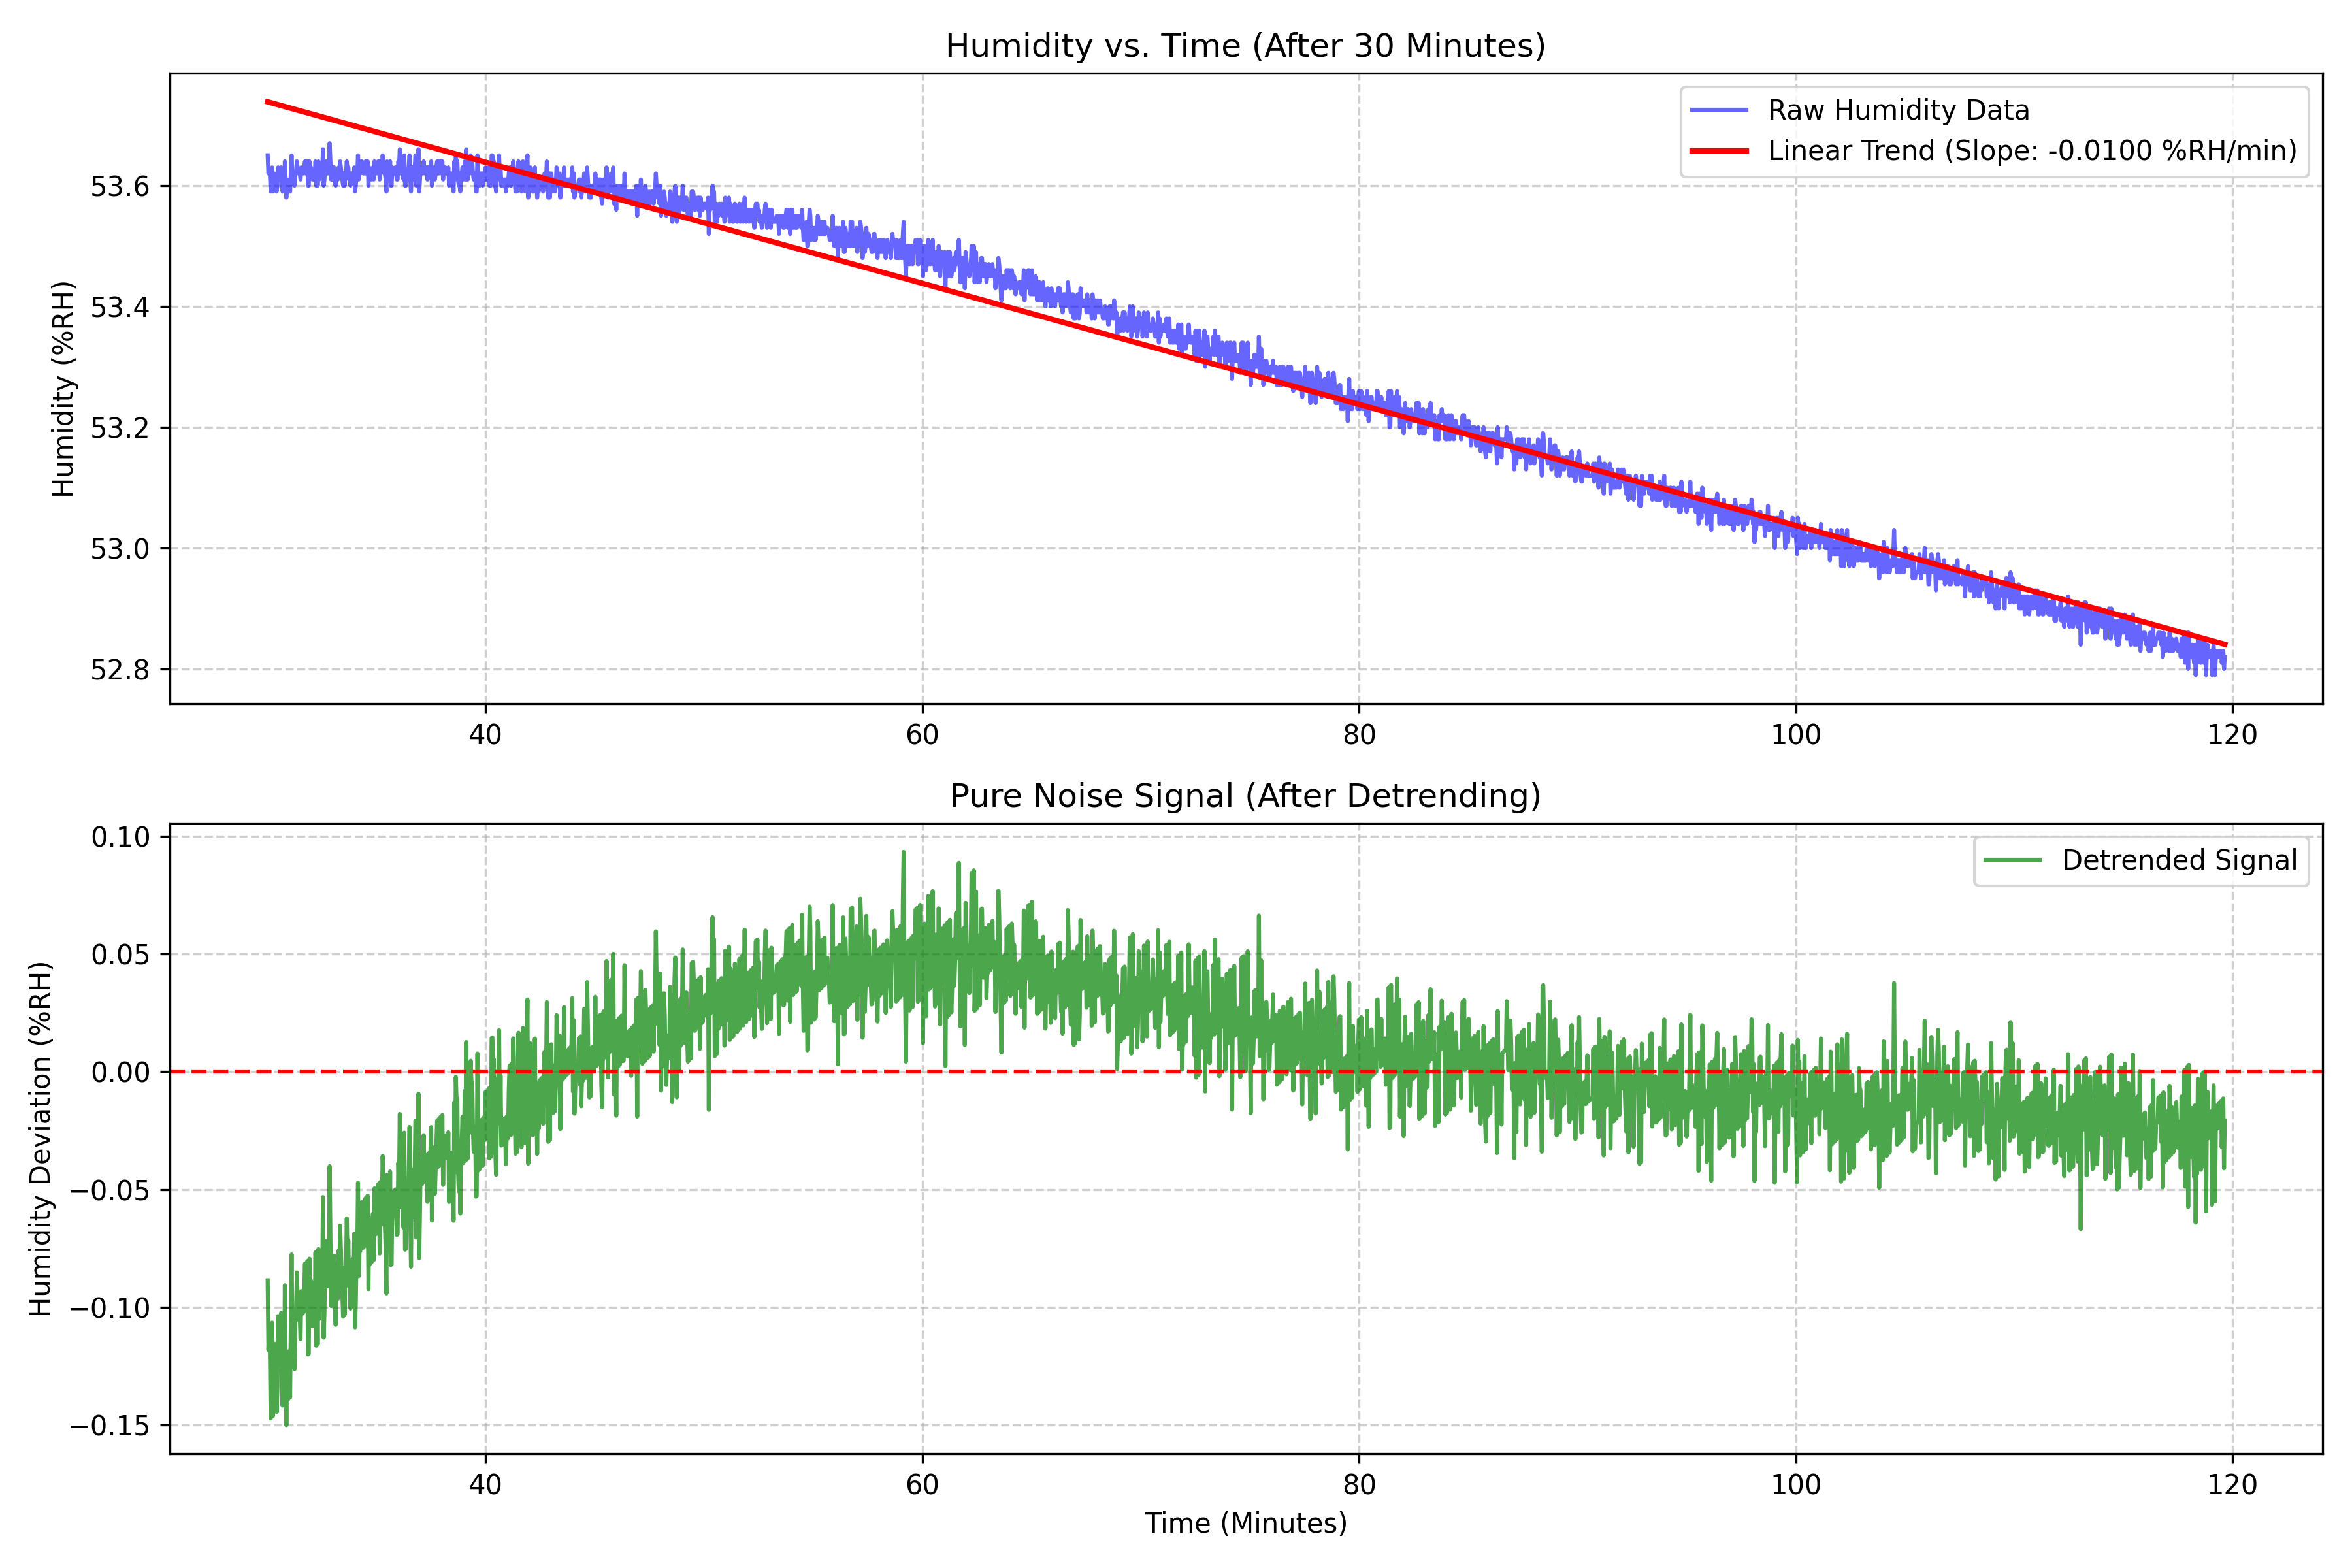
\includegraphics[width=\columnwidth]{./assets/RH/timeseries_plot.png}
\caption{Baseline time-series observation of the relative humidity channel demonstrating the inverse negative psychrometric drift.}
\label{fig:timeseries_RH}
\end{figure}

This behavior visually and mathematically confirms the inverse psychrometric relationship dictated by thermodynamics; 
at a constant absolute vapor pressure, an increase in sensible heat proportionally reduces relative humidity. 
Upon isolating this macroscopic drift via detrending, the true statistical means were established at $\mu_T = 30.7550^\circ$C and $\mu_{RH} = 53.2896$ \%RH, 
with isolated pure standard deviations (noise floors) of $\sigma_T = 0.0108^\circ$C and $\sigma_{RH} = 0.0370$ \%RH.

\subsection{Quantization Limits vs. Analog Front-End Noise}
To ascertain the physical origin of the measured uncertainty, 
the empirical noise floors were compared against the theoretical digital resolution of the sensor's 20-bit Analog-to-Digital Converter (ADC). 
The Least Significant Bit (LSB) quantization step for temperature is given by:
\begin{equation}
1 \text{ LSB}_T = \frac{200}{2^{20}} \approx 0.0001907^\circ\text{C}
\end{equation}
For the humidity channel, based on standard conversion parameters \cite{aht10_datasheet}, the resolution is:
\begin{equation}
1 \text{ LSB}_{RH} = \frac{100}{2^{20}} \approx 0.0000954\,\%\text{RH}
\end{equation}
The ratio of the measured noise floor to the quantization step demonstrates that the physical noise is $56.8\times$ larger than the digital limit for temperature ($0.0108 / 0.0001907$), 
and a substantial $388\times$ larger for humidity ($0.0370 / 0.0000954$). 
This strong quantitative evidence suggests that the precision bottleneck is primarily governed by the analog front-end (the capacitive polymer and silicon architecture) and thermodynamic fluctuations, rather than the digital bit depth. 
Consequently, transmitting raw, unfiltered data introduces severe measurement uncertainty, supporting the necessity of dedicated digital signal conditioning.

\subsection{EMA Filter Optimization via Cost Function}
Given the disparate physical properties of heat transfer versus moisture diffusion, 
the filter parameters required independent mathematical optimization. 
Evaluation of the objective function $J(\alpha)$ defined in \eqref{eq:cost_func} yielded distinct parabolic minima for each physical channel.

\begin{figure}[htbp]
\centering

\includegraphics[width=\columnwidth]{./assets/T/cost_function_optimization.png}
\caption{Cost function minimization for the temperature channel, indicating an optimal $\alpha_T = 0.1494$.}
\label{fig:cost_T}
\end{figure}

\begin{figure}[htbp]
\centering
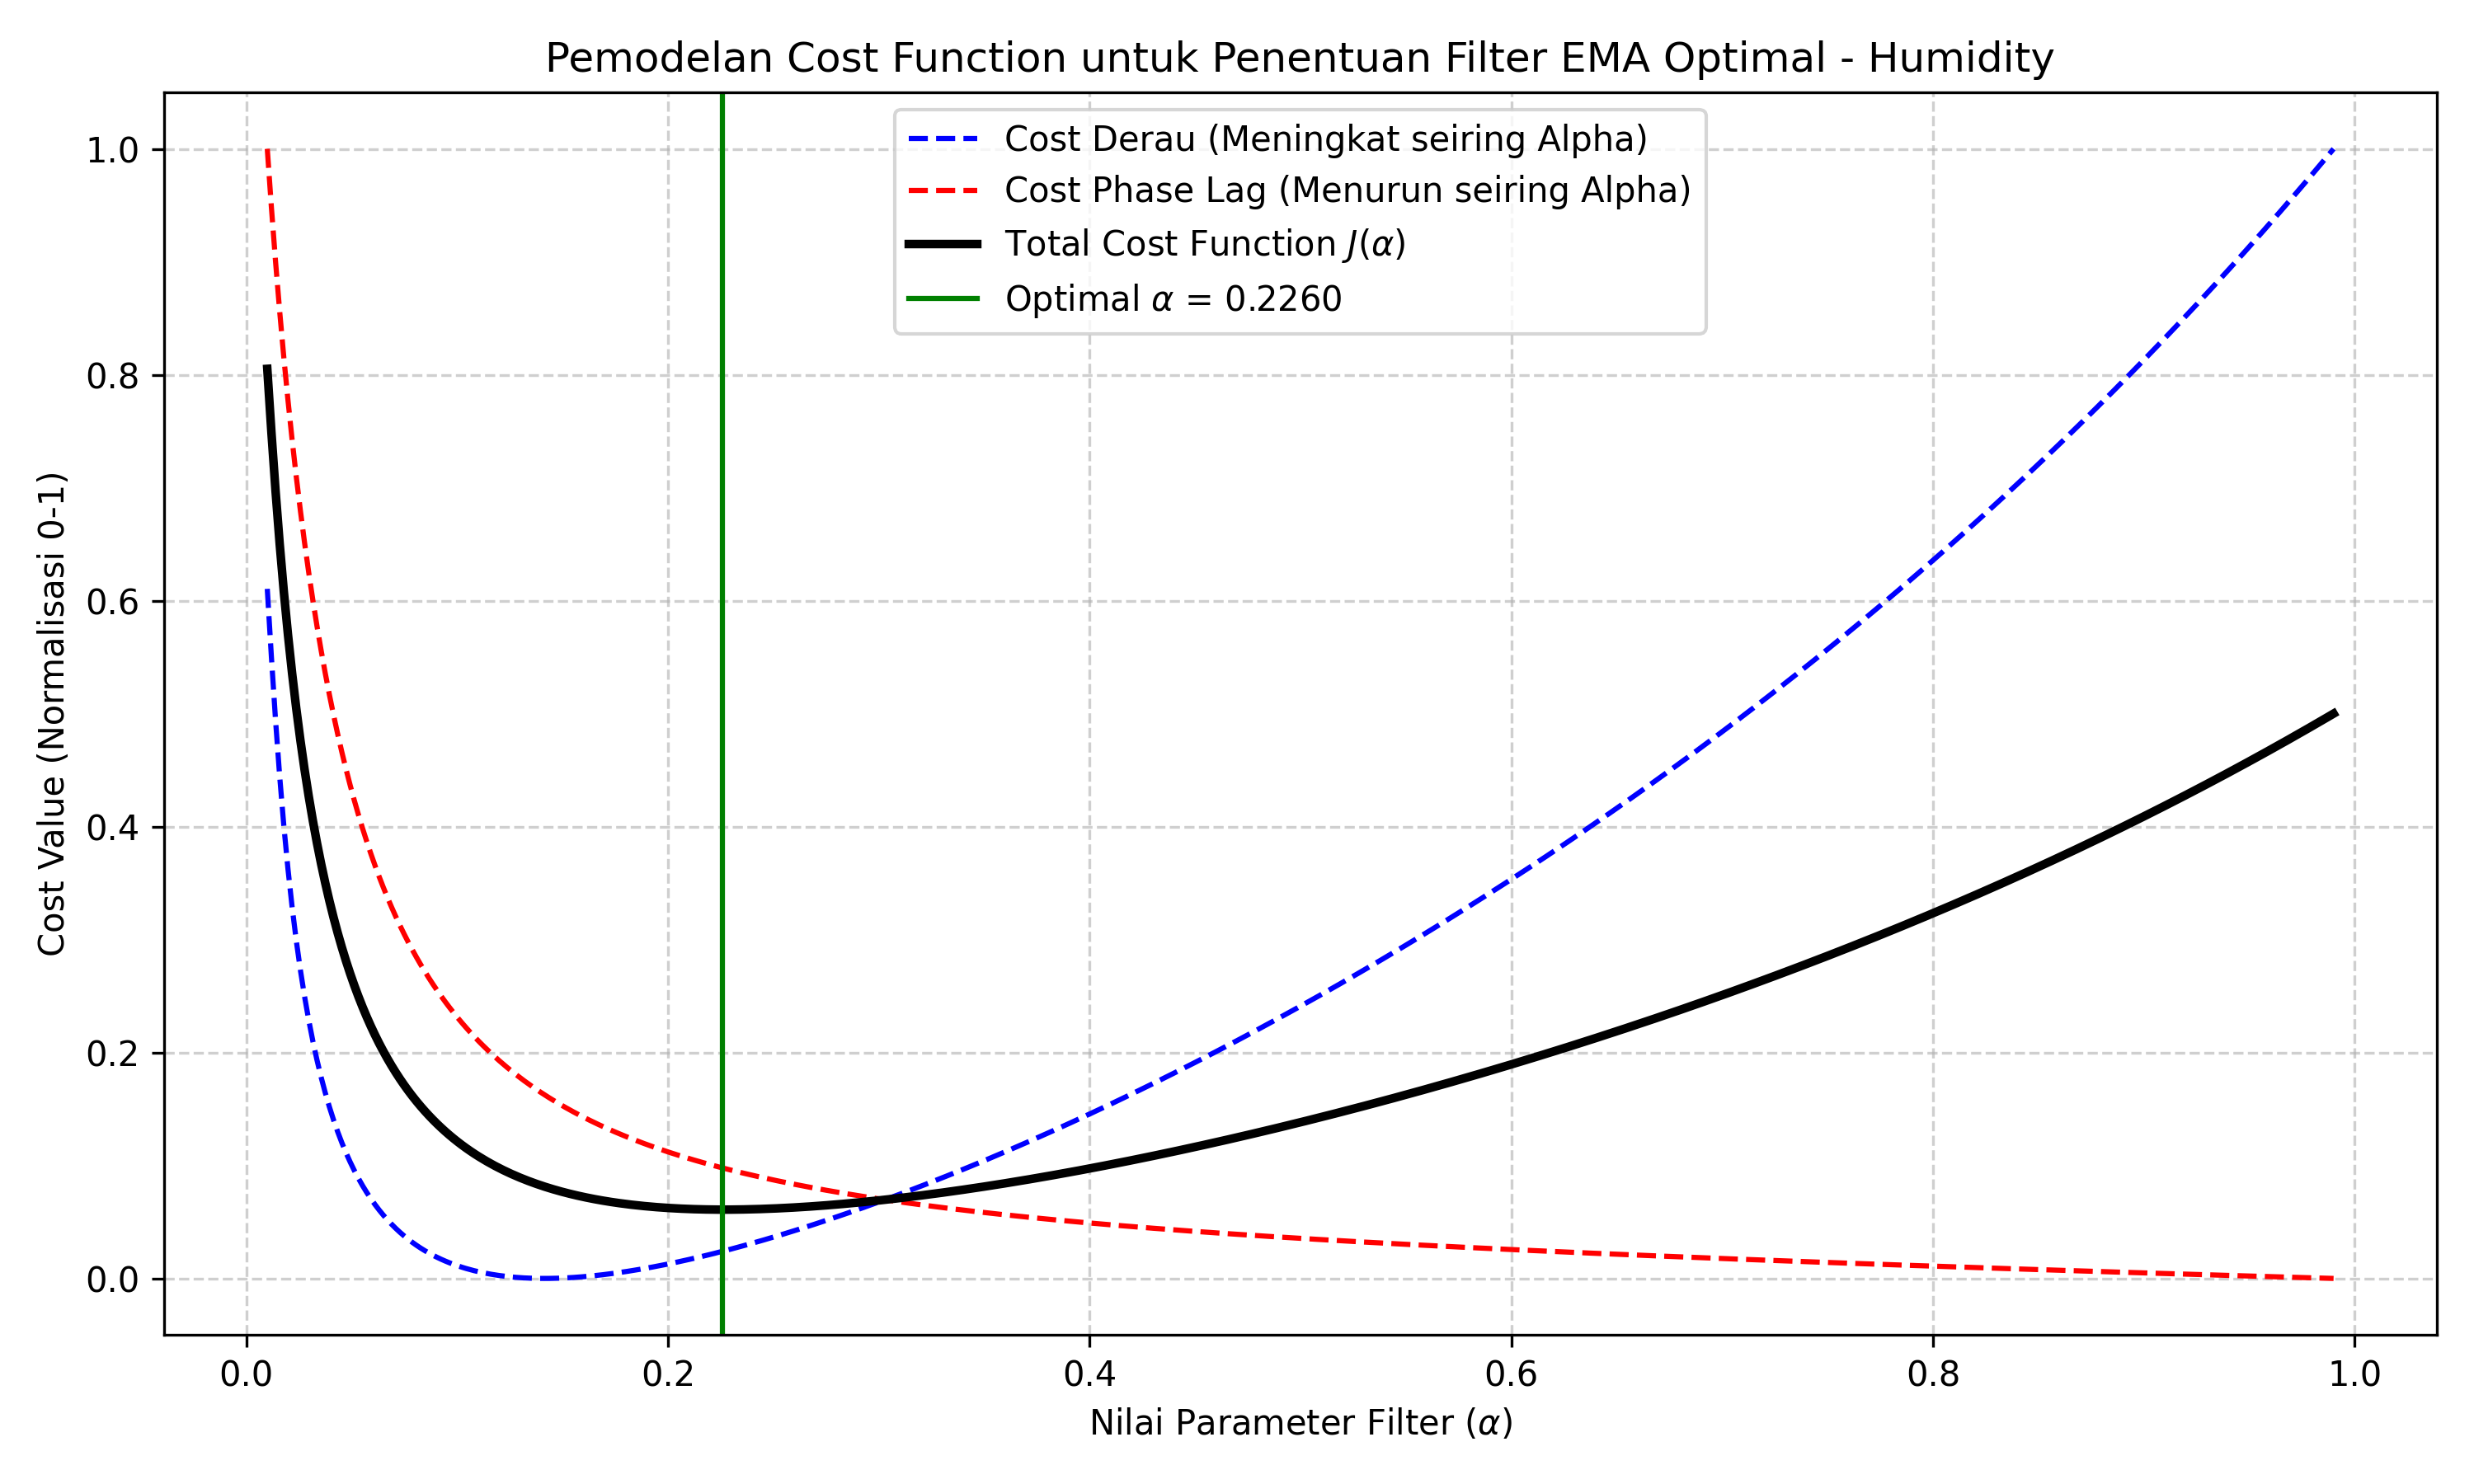
\includegraphics[width=\columnwidth]{./assets/RH/cost_function_optimization.png}
\caption{Cost function minimization for the relative humidity channel, indicating an optimal $\alpha_{RH} = 0.2260$.}
\label{fig:cost_RH}
\end{figure}

The baseline penalty weights ($W_1 = W_2 = 0.5$) utilized in the Cost Function were established under a neutral parity assumption, 
granting equal priority to steady-state noise suppression and transient response fidelity for environmental data-logging applications. 
While advanced multi-objective frameworks (such as Pareto fronts or Bayesian optimization) could map broader weighting trajectories, 
a balanced parity baseline provides a clear and reproducible design starting point. 
Under this configuration, as depicted in Fig. \ref{fig:cost_T} and Fig. \ref{fig:cost_RH}, numerical minimization established the optimal smoothing factors at $\alpha_T = 0.1494$ and $\alpha_{RH} = 0.2260$. 
The significantly higher $\alpha$ value for the RH channel reflects the faster intrinsic transient dynamics of humidity within this experimental boundary, allowing for more aggressive smoothing without proportionally sacrificing phase lag. 
The optimized filter parameters yield a theoretical noise standard deviation ($\sigma$) reduction of $71.6\%$ (corresponding to a $91.9\%$ variance attenuation) for temperature, and $64.3\%$ ($87.3\%$ variance attenuation) for humidity.

To rigorously test the stability and responsiveness of the optimization framework against shifting design priorities, 
a sensitivity analysis was conducted by adjusting the penalty weights to prioritize transient response fidelity ($W_1 = 0.3$ for noise variance and $W_2 = 0.7$ for phase lag). 
Executing the numerical minimization under this lag-prioritized configuration shifted the optimal smoothing factors upward to $\alpha_T = 0.2555$ for temperature and $\alpha_{RH} = 0.2967$ for relative humidity. 
This systematic upward migration mathematically confirms the elasticity of the Cost Function: as the operational penalty for transient delay increases, the system autonomously increases $\alpha$ to track rapid physical changes more aggressively, 
demonstrating that the framework can be seamlessly tailored to alternative embedded architectures (such as closed-loop control systems).

\subsection{Quantitative Evaluation of Phase Lag}
The transient phase lag was quantitatively evaluated across a critical temporal window (Minutes 3.0 to 6.0) following the physical step input.

\begin{figure}[htbp]
\centering

\includegraphics[width=\columnwidth]{./assets/T/transient_overall_plot.png}
\caption{Overall transient response of the temperature channel post-injection.}
\label{fig:transient_T}
\end{figure}

\begin{figure}[htbp]
\centering
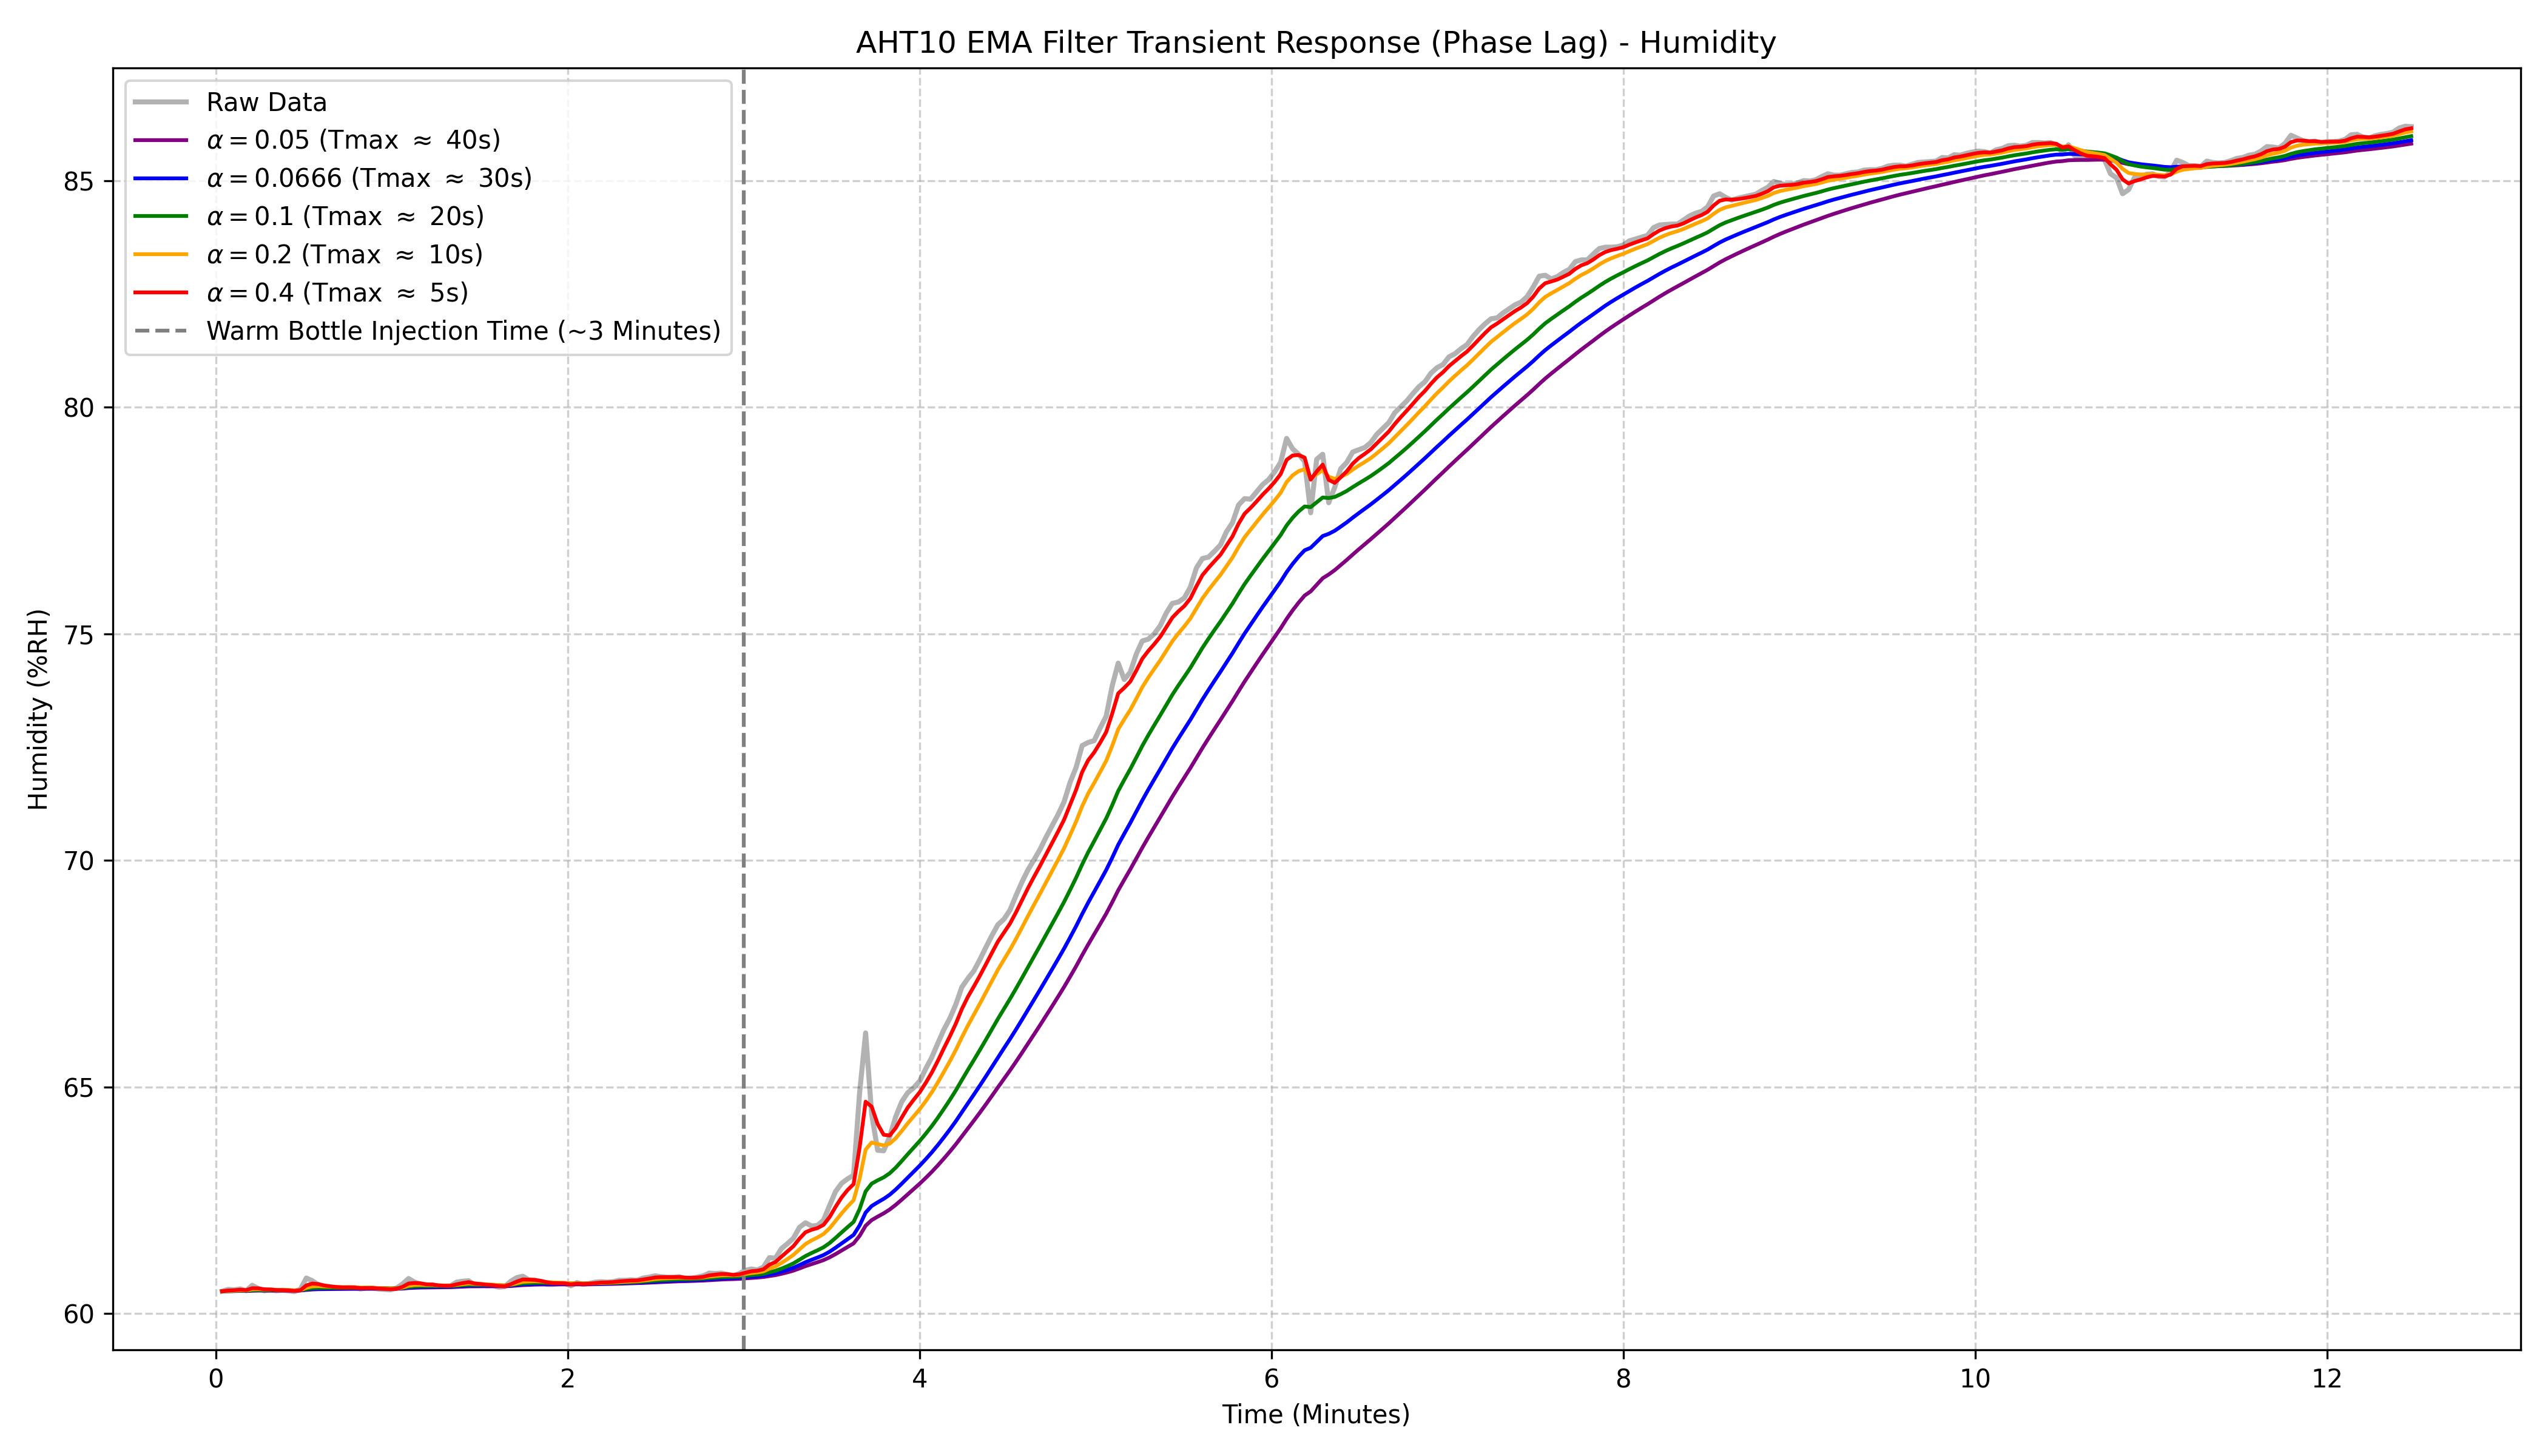
\includegraphics[width=\columnwidth]{./assets/RH/transient_overall_plot.png}
\caption{Overall transient response of the relative humidity channel post-injection.}
\label{fig:transient_RH}
\end{figure}

Applying $\alpha_T = 0.1494$ reduced the Root Mean Square Error (RMSE) to $0.0771^\circ$C with a Maximum Lag Error of $0.1333^\circ$C, occurring at exactly $3.39$ minutes post-injection (Fig. \ref{fig:transient_T}). 
For humidity (Fig. \ref{fig:transient_RH}), applying $\alpha_{RH} = 0.2260$ yielded an RMSE of $0.7560$ \%RH and a Max Lag of $2.3984$ \%RH, locking at $3.69$ minutes. 
The locking of maximal lag early in the transient window confirms the characteristic low-pass behavior of the filter in absorbing initial shock responses before adapting to the continuous physical change.

Translating these discrete variables into continuous physical time constants ($\tau$) using the relationship $\tau = -\Delta t / \ln(1-\alpha)$ yields $\tau_T \approx 12.67$\,s and $\tau_{RH} \approx 8.00$\,s. 
Crucially, the empirically derived $\tau_{RH}$ is mathematically identical to the intrinsic ``typical response time'' ($t_{63\%} = 8$\,s) specified by the AHT10 manufacturer \cite{aht10_datasheet}. 
Concurrently, $\tau_T$ falls perfectly within the established $5$--$30$\,s limit for thermal response. 
This serves as a definitive cross-validation: the objective, data-driven optimization of the cost function independently converged upon the physical thermodynamic limits of the hardware itself.

\subsection{Experimental Limitations and Gap Analysis}
While the empirical models present robust cross-validation against the physical hardware specifications, the methodological framework contains intrinsic metrological limitations. 

First, the deterministic hardware polling interval ($\Delta t = 2.051$\,s), while vital to strictly cap the SoC Joule heating below $0.1^\circ$C, limits the Nyquist frequency to $f_N \approx 0.243$\,Hz. 
Consequently, any high-frequency microclimate turbulence exceeding this limit cannot be reconstructed and will alias into the baseband, representing a deliberate design compromise that prioritizes long-term thermal stability over high-frequency dynamic capture.

Second, the physical transient injection utilized in Protocol II (warm water at $40^\circ$C--$50^\circ$C) deviates from an ideal mathematical Heaviside step function. 
The finite heat transfer rate dictates the temperature gradient, preventing an instantaneous physical change. 
Furthermore, the injection introduces not only sensible heat but also latent heat in the form of water vapor. 
This instantaneous surge in absolute humidity induces microscopic condensation on the AHT10's capacitive polymer membrane, where subsequent mechanical absorption and desorption phases introduce a physical inertia that overlaps with algorithmic phase lag. 
Therefore, the recorded RMSE and Max Lag Error metrics reflect the specific boundary constraints of this experimental setup and the sensor's mechanical membrane inertia. 

Finally, regarding the objective optimization framework, the baseline parity assumption ($W_1 = W_2 = 0.5$) provides a balanced starting point for environmental data logging. 
Preliminary sensitivity evaluations indicate that shifting the weights (e.g., favoring noise reduction with $W_1 = 0.7, W_2 = 0.3$) yields a more conservative smoothing factor ($\alpha$ decreases), reducing steady-state variance at the expense of a prolonged transient time constant. 
Future investigations could extend this optimization via multi-objective Pareto mapping, expand the metrological pipeline across alternative multi-sensor architectures (e.g., BME280, SHT31), and incorporate Type A/B expanded uncertainty frameworks to generalize these findings further.


\section{Conclusion}
This study rigorously characterized the noise profile and transient response dynamics of the AHT10 sensor through a strictly deterministic, localized data acquisition protocol. 
By explicitly disabling wireless hardware interrupts and applying linear detrending, the true analog noise floor was successfully isolated. 
A direct mathematical comparison against the 20-bit digital quantization boundaries strongly indicates that signal uncertainty is dominated by analog front-end noise, exceeding the theoretical LSB limit by factors of $56.8\times$ for temperature and $388\times$ for relative humidity. 

To condition the signal effectively while preserving temporal fidelity, a calculus-based Cost Function was deployed to numerically optimize independent Exponential Moving Average filters. 
The resulting parameters, $\alpha_T = 0.1494$ and $\alpha_{RH} = 0.2260$, demonstrate that disparate physical mechanisms—thermal inertia and moisture diffusion—mandate independent signal processing configurations. 
Furthermore, the convergence of the optimized time constant ($\tau_{RH} \approx 8.00$\,s) with the sensor's published physical hardware specifications successfully validates the employed mathematical framework, ensuring optimal preservation of both transient accuracy and steady-state precision in metrological evaluations.

\bibliographystyle{IEEEtran}
\bibliography{references}

\end{document}
